\section{Results}
\label{sec:results}

\subsection{Structural Sparsity Reduces Charged Complexity}
Table~\ref{tab:structural_overall} summarizes the 30-series development ablation under validation-RMSE selection. Fixed-$K$ TSK has the largest randomized dimension, KL, and certificate. Radius control reduces the mean rule count from 12 to 3.80 and the mean dimension from 135.6 to 39.7.

\begin{table}[t]
\centering
\caption{Development ablation over 30 synthetic series. Models are selected by validation RMSE; lower values are better.}
\label{tab:structural_overall}
\small
\setlength{\tabcolsep}{3.2pt}
\begin{tabular}{lrrrr}
\toprule
Family & $\bar K$ & $\bar D$ & Gaussian KL & Certificate \\
\midrule
Ridge & 1.00 & 13.4 & 5.16 & 0.1145 \\
Fixed-$K$ TSK & 12.00 & 135.6 & 39.55 & 0.2221 \\
Radius TSK & 3.80 & 39.7 & 16.63 & 0.1589 \\
Radius Top-3 TSK & 3.57 & 40.2 & 16.83 & 0.1589 \\
\bottomrule
\end{tabular}
\end{table}

\begin{table}[t]
\centering
\caption{Paired Radius-TSK minus Fixed-$K$-TSK differences over 30 development series. Negative values favor Radius TSK.}
\label{tab:structural_pairwise}
\small
\setlength{\tabcolsep}{4pt}
\begin{tabular}{lrr}
\toprule
Metric & Mean difference & Radius lower \\
\midrule
Dimension & -95.9 & 29/30 \\
Gaussian KL & -22.917 & 27/30 \\
Certificate & -0.0631 & 28/30 \\
Test RMSE & -0.0335 & 24/30 \\
\bottomrule
\end{tabular}
\end{table}


The paired differences in Table~\ref{tab:structural_pairwise} establish the contrast with the originally prespecified dense $K=12$ baseline. Relative to that baseline, radius-controlled all-active TSK reduces dimension by 95.9 coefficients, Gaussian KL by 22.917, and certificate value by 0.0631 on average. Its certificate is tighter in 28 of 30 series and its test RMSE is lower in 24 of 30. This comparison shows the cost of an unnecessarily dense rule base, but it does not by itself establish that radius selection is superior to a well-chosen smaller fixed $K$.

By contrast, Top-3 activation does not materially change the certificate. Across 5,600 matched candidate pairs, the mean Top-3 minus all-active certificate difference is approximately $-5\times10^{-5}$, and the selected-family averages in Table~\ref{tab:structural_overall} are effectively identical. Since Top-3 does not reduce $K(p+1)$, it should be described as a computational approximation, not the source of the PAC-Bayesian complexity gain.

\begin{figure}[t]
\centering
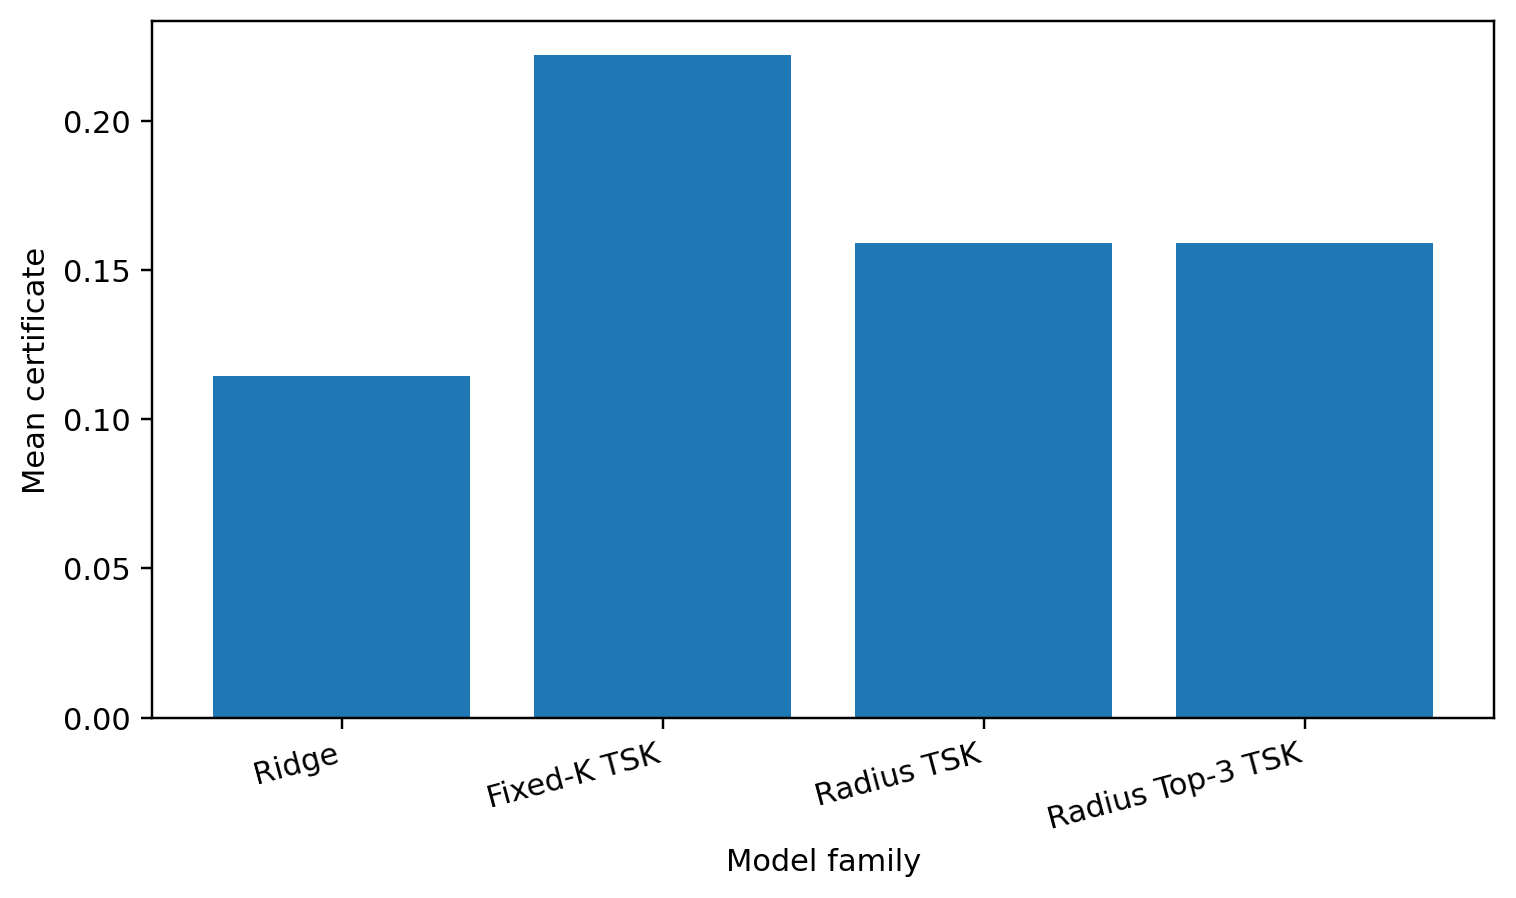
\includegraphics[width=\columnwidth]{figures/structural_certificate_by_family.png}
\caption{Mean familywise certificate under validation-RMSE selection across 30 synthetic development series. Ridge is tightest; radius control substantially improves on the originally prespecified fixed $K=12$ TSK baseline.}
\label{fig:structural_cert}
\end{figure}


\subsection{Fixed-$K$ Sensitivity Qualifies the Radius Advantage}
\begin{table}[t]
\caption{Fixed-$K$ sensitivity under validation-RMSE selection across 30 synthetic development series. The paired difference is Radius TSK minus Fixed-$K$ TSK; negative values favor radius control.}
\label{tab:fixed_k_sensitivity}
\centering
\footnotesize
\begin{tabular}{rrrrrr}
\toprule
$K$ & Dimension & Gaussian KL & Certificate & Test RMSE & $\Delta$ Cert. \\
\midrule
2 & 23.7 & 10.180 & 0.1326 & 0.8850 & +0.0264 \\
3 & 34.3 & 13.469 & 0.1465 & 0.8846 & +0.0125 \\
4 & 41.9 & 17.294 & 0.1568 & 0.8869 & +0.0021 \\
6 & 60.0 & 21.011 & 0.1701 & 0.8950 & -0.0112 \\
8 & 82.9 & 26.413 & 0.1875 & 0.8951 & -0.0286 \\
12 & 135.6 & 39.547 & 0.2221 & 0.9149 & -0.0631 \\
\bottomrule
\end{tabular}
\end{table}


Table~\ref{tab:fixed_k_sensitivity} shows that the mean fixed-$K$ certificate increases steadily with rule count, from 0.1326 at $K=2$ to 0.2221 at $K=12$. The radius-controlled mean is 0.1589. Consequently, radius control is not uniformly tighter than fixed rule bases: its mean certificate is looser than fixed $K=2$ and $K=3$, essentially matched by $K=4$, and tighter than the larger $K=6,8,12$ alternatives. After Holm correction, the paired certificate advantage is clear for $K=8$ and $K=12$, while the differences for $K=3,4,6$ are not statistically decisive.

When each series is allowed to choose its best fixed $K$ by validation RMSE, radius control changes the certificate by only $-0.0068$ on average (radius minus best fixed $K$; 95\% bootstrap interval $[-0.0187,0.0049]$) and the paired Wilcoxon result is not significant after correction. The corresponding test-RMSE difference is $-0.0054$ with bootstrap interval $[-0.0118,-0.0002]$, but the rank test is again not significant after multiplicity correction. Nine of 30 series select $K=2$, five select $K=3$, four select $K=4$, six select $K=6$, five select $K=8$, and only one selects $K=12$. Under certificate selection, all 30 series select fixed $K=2$.

These results materially narrow the structural claim. Radius construction is useful as an adaptive mechanism that avoids large unnecessary rule bases, but the certificate gain relative to $K=12$ is mainly a rule-count effect. The current evidence does not show that radius control dominates a predeclared and fairly charged small fixed-$K$ grid.

\begin{figure}[t]
\centering
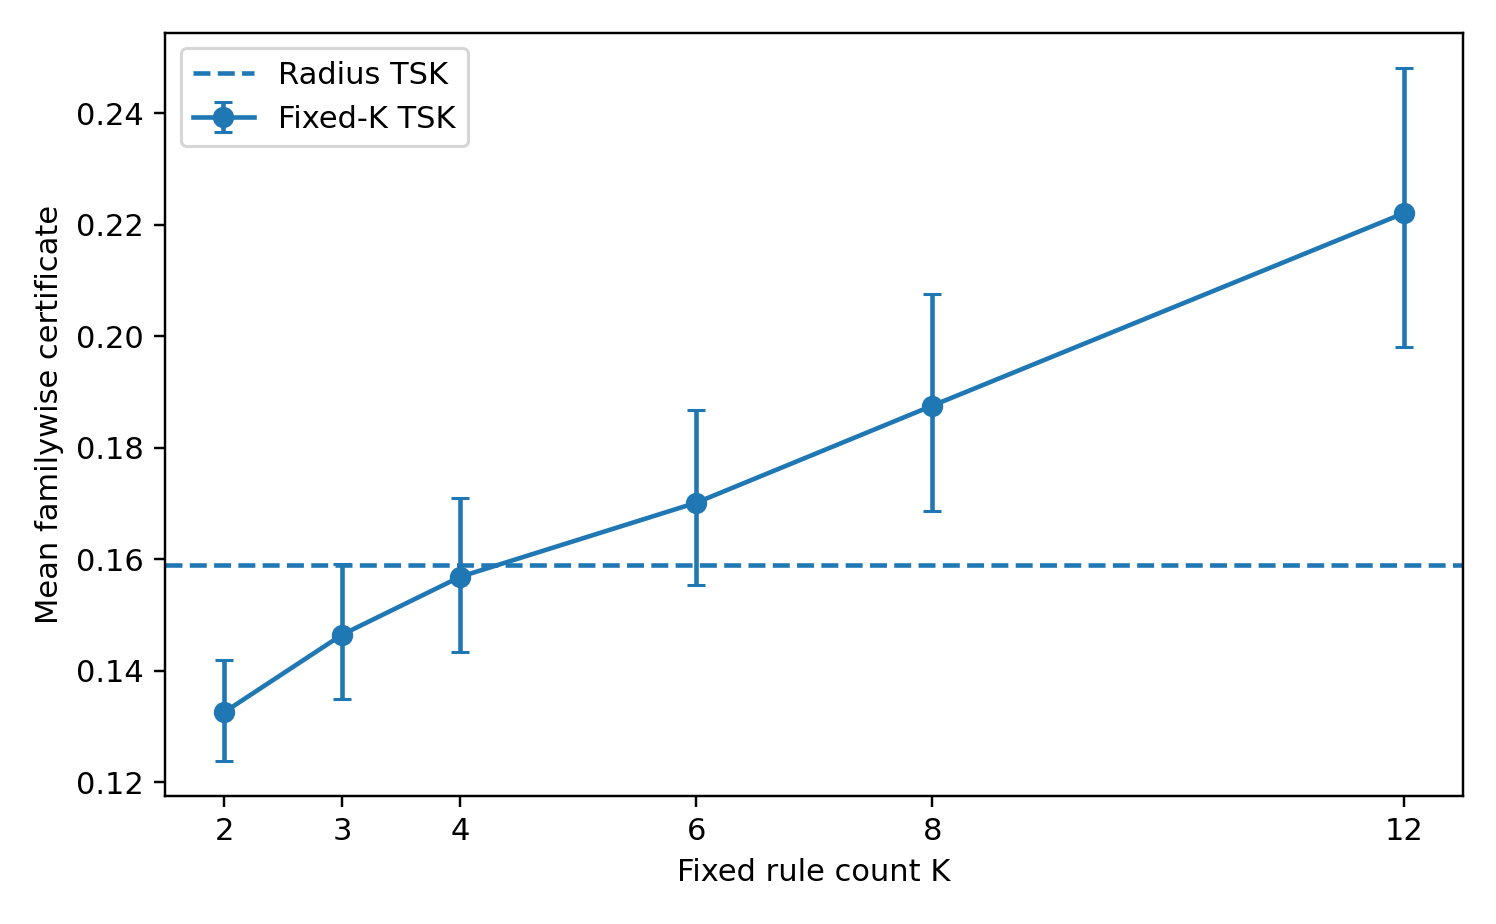
\includegraphics[width=\columnwidth]{figures/fixed_k_certificate_sensitivity.png}
\caption{Mean familywise certificate for fixed-$K$ TSK under validation-RMSE selection. Error bars are bootstrap intervals for the per-series means; the dashed line is the radius-controlled TSK mean.}
\label{fig:fixed_k_sensitivity}
\end{figure}

\begin{figure}[t]
\centering
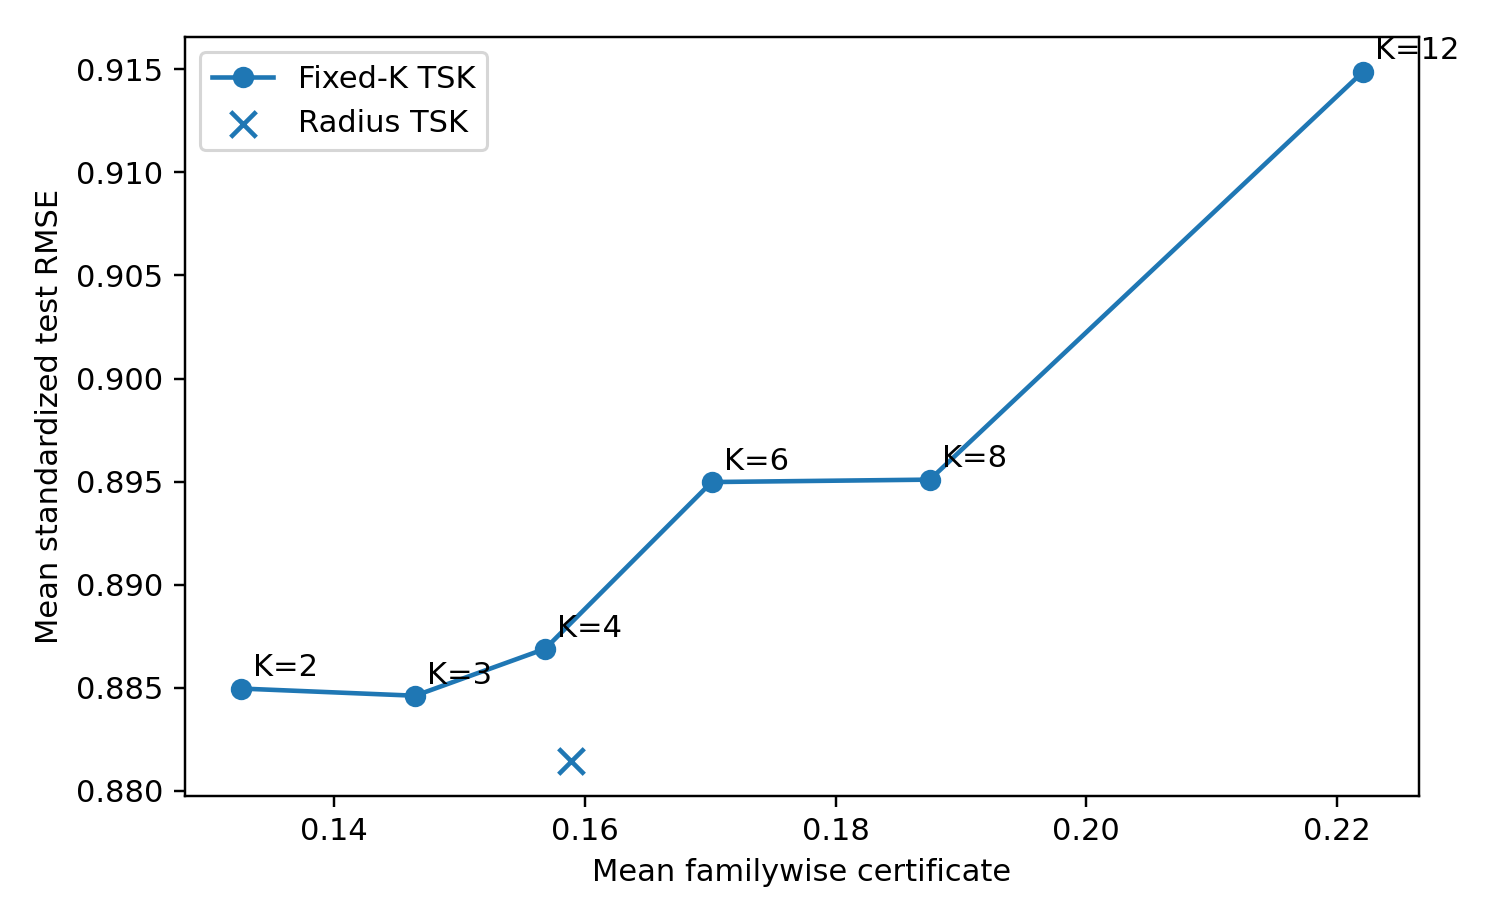
\includegraphics[width=\columnwidth]{figures/fixed_k_pareto_sensitivity.png}
\caption{Development mean test RMSE versus mean familywise certificate across fixed rule counts and radius-controlled TSK. The plot is descriptive and does not imply a universal Pareto ordering.}
\label{fig:fixed_k_pareto}
\end{figure}

\subsection{The Radius--Rule--Dimension--KL Chain}
Within each process, family, and lag, Spearman correlations across radius values average $-0.847$ for radius versus rule count, $1.000$ for rule count versus dimension, $0.981$ for dimension versus Gaussian KL, and $0.982$ for Gaussian KL versus certificate. These are descriptive associations rather than a universal monotonicity theorem, but they make the realized complexity path observable:
\begin{equation}
r\longrightarrow K(r)\longrightarrow D(r)\longrightarrow \mathrm{KL}\longrightarrow \operatorname{Cert}.
\end{equation}

Ridge retains the smallest mean certificate under both selection strategies: 0.1145 under validation-RMSE selection and 0.1017 under certificate selection. The results therefore do not support a claim that TSK is intrinsically easier to certify than a linear model.

\subsection{Predictive Accuracy and Clipping}
\begin{table*}[t]
\centering
\caption{Synthetic development results selected by validation RMSE (five seeds per process). RMSE is on the prior-standardized scale.}
\label{tab:process_results}
\small
\setlength{\tabcolsep}{5pt}
\begin{tabular}{lrrrrrr}
\toprule
& \multicolumn{2}{c}{Test RMSE} & \multicolumn{2}{c}{Certificate} & \multicolumn{2}{c}{Target clipping} \\
\cmidrule(lr){2-3}\cmidrule(lr){4-5}\cmidrule(lr){6-7}
Process & Ridge & Radius TSK & Ridge & Radius TSK & Cert. & Test \\
\midrule
AR(2) & 0.9098 & 0.9126 & 0.1128 & 0.1271 & 0.62\% & 0.35\% \\
SETAR & 1.0140 & 0.9798 & 0.1131 & 0.1467 & 0.42\% & 0.50\% \\
NARMA-10 & 0.7670 & 0.7656 & 0.1093 & 0.1188 & 0.97\% & 0.30\% \\
Mackey--Glass & 0.0656 & 0.0539 & 0.1129 & 0.2403 & 0.92\% & 1.30\% \\
GARCH & 1.0398 & 1.0926 & 0.0941 & 0.1114 & 0.25\% & 0.20\% \\
Structural break & 1.5236 & 1.4841 & 0.1445 & 0.2093 & 23.87\% & 71.55\% \\
\bottomrule
\end{tabular}
\end{table*}


Table~\ref{tab:process_results} separates predictive accuracy from certificate tightness. Radius TSK improves mean test RMSE over ridge on SETAR, NARMA-10, Mackey--Glass, and the structural-break process, but is slightly worse on AR(2) and materially worse on GARCH. Its largest benefit is Mackey--Glass, where mean RMSE falls from 0.0656 to 0.0539, while its certificate is more than twice the ridge value because of additional complexity.

The structural-break process is a failure-boundary example. Certification target clipping is 23.87\% and test target clipping is 71.55\%. The bounded certificate remains formally meaningful for the clipped loss, but it is not an operational description of raw errors after the break.

The localized prior improves the selected familywise certificate over a zero-mean prior in 85.6\% of selected rows, with mean absolute improvement 0.0138 after charging the same prior-variant mixture cost. Localization is useful but not uniformly superior; GARCH contains counterexamples.

\subsection{Negative Tetouan Development Outcome}
The initial Tetouan gate admits a radius TSK model in zone 1 and a fixed-$K$ TSK model in zone 2, while zone 3 abstains. Both learned deployments fail on the test horizon: RMSE changes are $-11.86\%$ and $-1.51\%$, and asymmetric-cost changes are $-22.67\%$ and $-19.05\%$. Averaged over all three zones, including the zone-3 fallback, RMSE worsens by 4.46\% and cost worsens by 13.91\%.

This negative result demonstrates that a non-vacuous certificate plus overall validation performance is not a sufficient deployment rule under temporal shift. It motivated the stricter margin and block-stability requirements in the independent confirmatory protocol.

\subsection{Independent PJM Confirmatory Outcome}
\begin{table*}[t]
\centering
\caption{Operational decision studies. Improvements are relative to the predeclared seasonal-naive fallback; negative values indicate degradation.}
\label{tab:energy_decisions}
\small
\setlength{\tabcolsep}{4pt}
\begin{tabular}{lllr rr}
\toprule
Phase & Series & Deployment & Certificate & Test RMSE imp. & Test cost imp. \\
\midrule
Tetouan dev. & zone 1 & dense\_tsk & 0.1226 & -11.86\% & -22.67\% \\
Tetouan dev. & zone 2 & fixed\_k\_dense\_tsk & 0.1482 & -1.51\% & -19.05\% \\
Tetouan dev. & zone 3 & seasonal\_naive\_24h & -- & 0.00\% & 0.00\% \\
\midrule
PJM confirm. & AEP & ridge & 0.0959 & 57.97\% & 58.64\% \\
PJM confirm. & COMED & ridge & 0.0841 & 55.40\% & 54.11\% \\
PJM confirm. & DAYTON & dense\_tsk & 0.0933 & 49.13\% & 50.30\% \\
PJM confirm. & PJME & ridge & 0.0959 & 51.70\% & 51.42\% \\
\bottomrule
\end{tabular}
\end{table*}


The frozen PJM gate admits a learned model in all four regions. Test RMSE improves by 57.97\%, 55.40\%, 49.13\%, and 51.70\% for AEP, COMED, DAYTON, and PJME, respectively. Corresponding asymmetric-cost improvements are 58.64\%, 54.11\%, 50.30\%, and 51.42\%; mean improvements are 53.55\% and 53.62\%. Selected certificates range from 0.0841 to 0.0959, and test target and forecast clipping are zero.

\begin{figure}[t]
\centering

\includegraphics[width=\columnwidth]{figures/pjm_test_improvements.png}
\caption{Independent PJM test improvements over the frozen seven-day seasonal-naive fallback.}
\label{fig:pjm_improvements}
\end{figure}

The confirmatory result does not establish nonlinear fuzzy superiority. AEP, COMED, and PJME select ridge. DAYTON selects a radius-controlled one-rule TSK with lag 14; with one rule, this is an affine predictor. No fixed-eight-rule TSK candidate passes the frozen gate. The operational evidence therefore supports a complexity-aware gate that can shrink to a simple model, not a claim that a multi-rule TSK system caused the gain.
